\section*{Preprocessing}

Data preprocessing is a vital step in any Machine Learning pipeline, and it is particularly meaningful when dealing with natural language. The fact is that natural language is inherently ambiguous, and in many NLP tasks, we care a lot about the quality of our data which has to be high enough in order to achieve good results. In this case, we tackled the Sentiment Analysis task on the Twitter dataset which consists of a collection of user tweets with their annotated sentiment (either positive or negative) and some additional information such as the tweet identifier, the author, etc ...\\

As the first step, we cleaned the dataset from all the columns and retained only those related to text and (ground truth) sentiment annotation. We even performed some minor transformations on class labels which were originally defined in \{0,4\} to have values in \{0,1\}.\\

\begin{figure}[h!t]
    \centering
    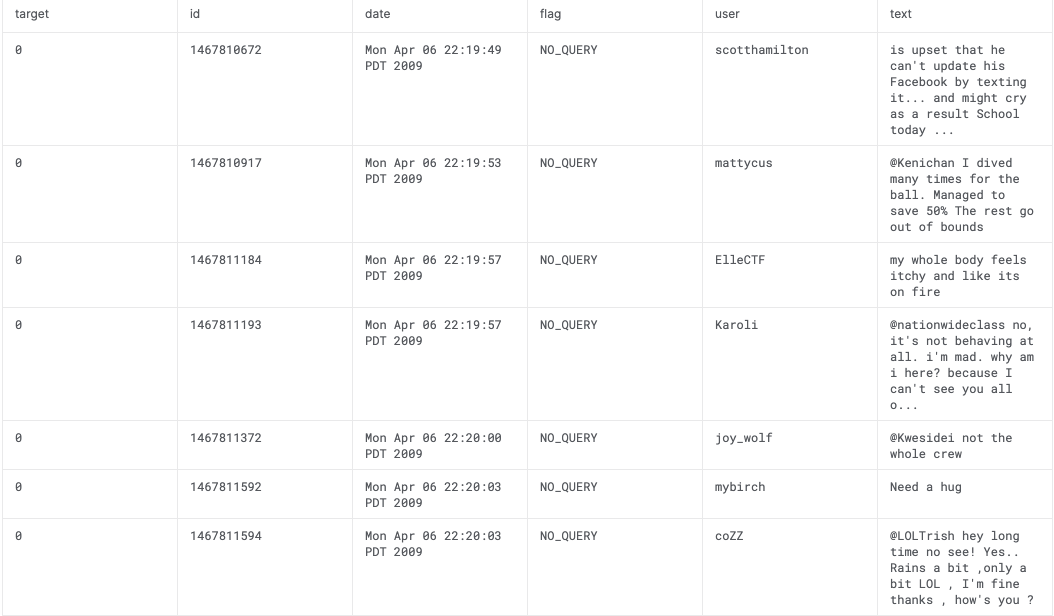
\includegraphics[width=11cm]{twitter_overview.png}
    \caption{Overview of the Twitter dataset.}
    \label{fig:TWITTER_OVERVIEW}
\end{figure}

We noticed that users tend to make mistakes when posting new tweets either because they contain typos (i.e. grammatical issues) or because they replace English words with abbreviations or idiomatical terms (i.e. slung or Internet jargon). Therefore, we chose to perform major treatments on our data and tried to correct these errors in order to enhance the quality of our corpus (e.g. replace duplicated characters, 'hellooo' becomes 'helloo' and 'tooo much' becomes 'too much').\\

We decided to apply lemmatization and tokenization, which are common operations in NLP tasks, on our dataset, and in order to do that we relied on the spaCy pipeline ~\cite{startups:spaCy} because of its efficiency and because nowadays many companies that deal with natural natural language processing have chosen to use it~\cite{data:companies_using_spacy}.\\

While it is common to tokenize sentences into words before passing them to a model, we thought it would be interesting to use lemmas instead of the original words since different variations of the original lemma have the same meaning (e.g. 'be', 'been' and 'am' refer to the same concept) and models should benefit from this process since they will have the chance to see multiple times the same lemma in different contexts. We also decided not to test the effects of applying stemming on our dataset since many stemming algorithms consider some heuristics to cut the end of a word, and while they can be successful in some occasions, this is not always the case ~\cite{data:standfordNLP}.\\

Moreover, we managed to filter out from our corpus those common words that do not contribute to adding meaning to our sentences: the so-called stopwords. There are a plethora of valid collections of stopwords available on the web (e.g. NLTK~\cite{startups:nltk}, Gensim~\cite{startups:gensim}) and we decided to use those offered by spaCy. Although stopwords removal is something very common in many NLP tasks, we later discovered that not all stopwords are equal and that there exist some stopwords that are more important than others. In other terms, the broader definition where all stopwords may be dropped when dealing with natural language may be more finely defined as a collection of frequently used words, whose presence does not in general add semantics to sentences, except for some cases (e.g. adversative conjunctions may be relevant in sentiment analysis).
Along these lines, we experimentally crafted a set of stopwords that allowed us to get better results. Please refer to the next sections for the relative discussion and the benchmarks.\\

However, the preprocessing phase was not something that was specifically designed for the Twitter dataset, and we applied it to all the datasets we compared with (e.g. IMDb~\cite{data:imdb}) when necessary.